%% ============================================================
%%  Вопрос 3: Различные определения деревьев
%% ============================================================
\section{Различные определения деревьев}

\subsection{Эквивалентные определения}

\begin{Statement}{Эквивалентные определения деревьев}{}
  Пусть $G=(V,E)$ — конечный неориентированный граф, $|V|=n$.
  Следующие утверждения эквивалентны:
  \begin{enumerate}
    \item[(i)]   $G$ — \emph{дерево} (связный ациклический граф).
    \item[(ii)]  Между любыми двумя вершинами $u,v\in V$ существует
                 ровно один простой путь.
    \item[(iii)] $G$ связен и $|E|=n-1$.
    \item[(iv)]  $G$ связен и при удалении любого ребра связность теряется.
  \end{enumerate}
\end{Statement}

\begin{proof}

  \subsubsection*{(i)$\Rightarrow$(ii)}

  Связность даёт существование пути.
  Если существуют два различных пути $u\to v$, их объединение содержит цикл
  — противоречие ацикличности.

  \subsubsection*{(ii)$\Rightarrow$(iv)}

  Возьмём ребро $e=xy$. В $G\setminus e$ не осталось пути между $x$ и $y$
  (иначе в $G$ их было бы два), поэтому удаление $e$ нарушает связность.

  \subsubsection*{(iv)$\Rightarrow$(i)}

  Если в $G$ есть цикл, ребро цикла можно удалить без нарушения связности
  (обход по остальной части цикла) — противоречие~(iv).
  Граф связен и ацикличен, то есть дерево.

  \subsubsection*{(i)$\Rightarrow$(iii)}

  Индукция по $n$. База $n=1$: $|E|=0=n-1$.
  Шаг: в любом дереве есть лист (см. ниже); удаляем его вместе с ребром —
  получаем дерево на $n-1$ вершинах с $|E|-1$ рёбрами.
  По ИП $|E|-1=(n-1)-1$, откуда $|E|=n-1$.

  \subsubsection*{(iii)$\Rightarrow$(i)}

  Если в связном графе $|E|=n-1$ есть цикл — удалим его ребро:
  граф останется связным, но $|E|=n-2 < n-1$ —
  невозможно (остовное дерево имеет $n-1$ ребро). Противоречие.
\end{proof}

\subsection{Листья}

\begin{Definition}{Лист}{}
  Вершина $u\in V$ дерева $G=(V,E)$ называется \emph{листом},
  если $\deg(u)=1$.
\end{Definition}

\begin{Statement}{}{}
  Если $G$ — дерево на $n\ge 2$ вершинах, то в $G$ есть хотя бы два листа.
\end{Statement}

\noindent
\begin{minipage}[t]{0.45\textwidth}
  \vspace{0pt}
  \centering
  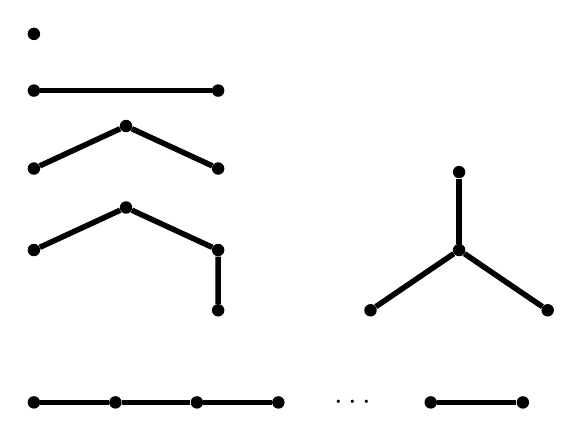
\begin{tikzpicture}[
    scale=0.45, transform shape,
    dot/.style={circle, fill=black, inner sep=0pt, minimum size=10pt},
    edge/.style={draw=black, line width=2pt}]

    \node[dot] at (0,7.2) {};

    \node[dot] (a) at (0,5.6) {};
    \node[dot] (b) at (5.2,5.6) {};
    \draw[edge] (a)--(b);

    \node[dot] (c1) at (0,3.4) {};
    \node[dot] (c2) at (2.6,4.6) {};
    \node[dot] (c3) at (5.2,3.4) {};
    \draw[edge] (c1)--(c2)--(c3);

    \node[dot] (d1) at (0,1.1) {};
    \node[dot] (d2) at (2.6,2.3) {};
    \node[dot] (d3) at (5.2,1.1) {};
    \node[dot] (d4) at (5.2,-0.6) {};
    \draw[edge] (d1)--(d2)--(d3)--(d4);

    \node[dot] (e0) at (12,1.1) {};
    \node[dot] (e1) at (12,3.3) {};
    \node[dot] (e2) at (9.5,-0.6) {};
    \node[dot] (e3) at (14.5,-0.6) {};
    \draw[edge] (e0)--(e1);
    \draw[edge] (e0)--(e2);
    \draw[edge] (e0)--(e3);

    \node[dot] (p0) at (0,-3.2) {};
    \node[dot] (p1) at (2.3,-3.2) {};
    \node[dot] (p2) at (4.6,-3.2) {};
    \node[dot] (p3) at (6.9,-3.2) {};
    \draw[edge] (p0)--(p1)--(p2)--(p3);

    \node at (9.0,-3.2) {\Huge$\cdots$};

    \node[dot] (q0) at (11.2,-3.2) {};
    \node[dot] (q1) at (13.8,-3.2) {};
    \draw[edge] (q0)--(q1);
  \end{tikzpicture}
\end{minipage}
\hfill
\begin{minipage}[t]{0.52\textwidth}
  \vspace{0pt}
  \textbf{Доказательство.}
  Пусть $\ell = |L|$, где $L$ — множество листьев.
  Так как $|E|=n-1$, по лемме о рукопожатиях
  \[
    \sum_{v\in V}\deg(v) = 2(n-1).
  \]
\end{minipage}

\medskip\noindent
Листья дают $\deg = 1$, остальные вершины — $\deg \ge 2$:
\[
  2(n-1) = \sum_{v}\deg(v) \ge \ell\cdot 1 + (n-\ell)\cdot 2 = 2n - \ell.
\]
Откуда $\ell \ge 2$. $\square$

\subsection{Остовные деревья и леса}

\begin{Theorem}{Существование остовного дерева}{}
  Если $G$ связен, из него можно удалить некоторые рёбра (без удаления вершин)
  так, чтобы получить дерево.
\end{Theorem}

\begin{proof}
  Пока в $G$ есть цикл, удаляем из него одно ребро:
  удаление ребра цикла не нарушает связность (обход по остатку цикла).
  Процесс конечен; в конце — связный ациклический граф, то есть дерево.
\end{proof}

\begin{Definition}{Остовное дерево}{}
  Подграф $T \subseteq G$ называется \emph{остовным деревом} графа $G$,
  если $T$ — дерево и $V(T)=V(G)$.
\end{Definition}

\begin{Definition}{Лес}{}
  Граф $F=(V,E)$ называется \emph{лесом}, если он не содержит циклов.
\end{Definition}

\begin{Statement}{Эквивалентные определения леса}{}
  Пусть $F=(V,E)$ — конечный граф, $c(F)$ — число компонент связности.
  Следующие утверждения эквивалентны:
  \begin{enumerate}
    \item[(i)]   $F$ не содержит циклов (лес);
    \item[(ii)]  $|E| = |V| - c(F)$;
    \item[(iii)] удаление любого ребра увеличивает число компонент;
    \item[(iv)]  каждая компонента связности $F$ является деревом.
  \end{enumerate}
\end{Statement}
